\documentclass[acmlarge]{acmart}

\setcopyright{acmcopyright}
\copyrightyear{2020}
\acmNumber{4}
\acmMonth{8}

\usepackage{listings}
\usepackage[section]{placeins}
\usepackage{multirow}
\usepackage{pgfplots}
\usepackage{yfonts}
\usepackage{subcaption}

\pgfplotsset{width=7cm,compat=1.8}

\lstdefinelanguage{ocanren}{
keywords={run, conde, fresh, let, in, match, with, when, class, type,
object, method, of, rec, until, while, not, do, done, as, val, inherit,
new, module, sig, deriving, datatype, struct, if, then, else, open, private, virtual, include, success, failure,
true, false},
sensitive=true,
commentstyle=\small\itshape\ttfamily,
keywordstyle=\textbf,%\ttfamily\underline,
identifierstyle=\ttfamily,
basewidth={0.5em,0.5em},
columns=fixed,
mathescape=true,
fontadjust=true,
literate={fun}{{$\lambda$}}1 {->}{{$\to$}}3 {===}{{$\equiv$}}1 {=/=}{{$\not\equiv$}}1 {|>}{{$\triangleright$}}3 {\\/}{{$\vee$}}2 {/\\}{{$\wedge$}}2 {^}{{$\uparrow$}}1,
morecomment=[s]{(*}{*)}
}

\lstset{
language=ocanren
}

\newcommand{\ruleno}[1]{\mbox{[\textsc{#1}]}}
\newcommand{\rulen}[1]{[\textsc{#1}]}
\newcommand{\mk}[0]{\textsc{miniKanren}}
\newcommand{\inbr}[1]{\langle #1 \rangle}

\begin{document}

\title{Fair relational conjunction}

\author{Petr Lozov}
\email{lozov.peter@gmail.com}        

\author{Dmitry Boulytchev}
\email{dboulytchev@math.spbu.ru}    

\affiliation{
  \institution{Saint Petersburg State University}
  \country{Russia}                   
}

\affiliation{
  \institution{JetBrains Research}   
  \country{Russia}                   
}

\begin{abstract}
  Abstract will be here.
\end{abstract}

\begin{CCSXML}
<ccs2012>
<concept>
<concept_id>10011007.10011006.10011008.10011009.10011015</concept_id>
<concept_desc>Software and its engineering~Constraint and logic languages</concept_desc>
<concept_significance>500</concept_significance>
</concept>
</ccs2012>
\end{CCSXML}

\ccsdesc[500]{Software and its engineering~Constraint and logic languages}

\keywords{relational programming, evaluation strategies}

\maketitle

\section{Introduction}

The Reasoned Schemer~\cite{fair:TheReasonedSchemer}

Quine Generation~\cite{fair:quines}

% Проблема несправедливого поведения конъюнкции уже рассматривалась с нескольких разных точек зрения.
The problem of unfair behavior of conjunction has already been examined from several different points of view.

% Одним из аспектов несправедливого поведения конъюнкции является управления приоритетами вычисления независимых ветвей, которые порождает конъюнкция. В оригинальном языке больший приоритет отдается более ранней ветке. Однако существует подход, который позволяет сбалансировать время исполнения. Это делает поведение конъюнкции более справедливым, но чувствительность к порядку конъюнктов сохраняется.
One aspect of the unfair behavior of a conjunction is to prioritize the evaluation of the independent branches that the conjunction generates. In the original \mk, a higher priority is given to an earlier branch. However, there is an approach~\cite{fair:towardsAM} that allows you to balance the time of the evaluation. This makes the conjunction behavior more fair, but the sensitivity to the order of the conjuncts remains.

% Также конъюнкция становится более честной, если детектировать расхождение конъюнктов. Данный подход во время исполнения может обнаружить расхождение конъюкта. В этом случае данные, которые были получены при исполнении конъюнкта стираются. После чего происходит перестановка конъюнктов и продолжается исполнение программы. Данный подход оказывается эффективен на практике. Недостатком является консервативная перестановка конъюнктов, которпя не использует информацию, полученную при вычислении конъюнкта до перестановки.
Also, the conjunction becomes more fair we will detect divergence of conjuncts. This approach~\cite{fair:DivTest} at run time can detect conjunct divergence. In this case, the data that was received during the evaluation of the conjunct is erased. After that there is a rearrangement of the conjuncts and the evaluation of the program continues. This approach is effective in practice. However, the conservative rearrangement of the conjuncts does not use the information obtained when evaluating the conjunct before the rearrangement.

\section{Directed relational conjunction}

% В этом разделе мы рассмотрим реляционный язык miniKanren с классической направленной конъюнкцией, изучим достоинства и недостатки направленной конъюнкции на примерах.
In this section we consider the relational language \mk~ with the classic directed conjunction and demonstrate the advantages and disadvantages of directed conjunction using examples. 

% В языке miniKanren между операциями дизъюнкции и конъюнкции есть существенная разница. Дизъюнкция вычисляет свои аргументы попеременно, что приводит к равномерному вычислению двух дизъюнктов. Такого поведения дизъюнкции достаточно для полного поиска ответов. Конъюнкция же извлекает ответы из первого конъюнкта, на которых вычисляет второй конъюнкт. С одной стороны, такая конъюнкция проста в реализации и позволяет явно задать порядок исполнения конъюнктов. С другой стороны, эта конъюнкция ассиметрична. Более того, она может сходиться при одном порядке конъюнктов, но расходиться при другом. Например, отнонение freeze в зависимости от аргумента либо сходится за один шаг рекурсии, либо расходится. Тогда конъюнкция вида (=== /\ freeze) сходится, но при перестановке конъюнктов мы получаем расхождение. Действительно, в первом случае первый конъюнкт производит ровно один ответ, который противоречит унификации в теле отношения freeze. Во втором случае отношение freeze разойдется и не произведет ни одного ответа и второй конъюнкт вычислен не будет. 
In classic \mk, there is a significant difference between disjunction and conjunction operations. 
The disjunction evaluates its arguments alternately, which leads to the uniform evaluation of two disjuncts. 
This behavior is enough to fully search for answers. 
The conjunction, on the other hand, extracts the answers from the first conjunct and it calculates the second conjunct using this answers.
On the one hand, this conjunction is easy to implement and allows you to explicitly specify the order of evaluation of the conjuncts.
On the other hand, this conjunction is asymmetric. 
Moreover, it can converge in one order of conjuncts, but diverge in another.
For example, relation
\begin{lstlisting}
let rec freeze$^o$ x = x ===  true /\ freeze$^o$ x
\end{lstlisting}
either converges in one recursion step or diverges.
Then conjunction \lstinline{(x === false/\ freeze$^o$ x)} converges, but conjunction with the reverse order of conjuncts \lstinline{(freeze$^o$ x /\ x === false)} diverges.
Indeed, in the first case, the first conjunct produces exactly one answer, which contradicts the unification in the body of the relation \lstinline{freeze$^o$}. In the second case, the relation \lstinline{freeze$^o$} diverges and isn't produce any answer. As a result, the second conjunct will not be evaluated.

% Конечно, данная проблема решается правилом, которому нужно следовать при работе с miniKanren: унификацию нужно ставить самым левым конъюнктом. Но иногда оба конъюнктв являются вызовами отношений. В частности отношение обращения списка revers, которое связывает произвольный список со списком, содержащим элементы в обратном порядке. В этом отношении есть пара конъюнктов append и revers. При таком порядке вызов revers сходится, но при обратном порядке он расходится. Более того при обратном порядке снижается скорость вычисления ответа. 
Of course, this problem can be solved by the rule that must be followed when working with \mk: unification must be the left-most conjunct.
But sometimes both conjuncts are calls of relations.
For instance, the relation \lstinline{revers$^o$} in figure~\ref{fair:lst-reverso}, which associates an arbitrary list with a list containing elements in reverse order.
In this relation we can see a couple of conjuncts: \lstinline{revers$^o$} in line~\ref{fair:reverso-call} and \lstinline{append$^o$} in line~\ref{fair:appendo-call}. In this order, the call \lstinline{(revers$^o$ [1, 2, 3] q)} converges, but in the reverse order it diverges after the answer is found. Moreover, the reverse order decreases the speed of evaluating the answer.

\begin{figure}[h]
\centering
\begin{tabular}{cp{3cm}c}
\begin{lstlisting}[numbers=left,numberstyle=\small]
let rec append$^o$ x y xy =
  (x === [] /\ y === xy) \/
  fresh (e xs xys) (
    x === e : xs /\ 
    xs === e : xys /\ 
    append$^o$ xs y xys)
\end{lstlisting}
& &
\begin{lstlisting}[firstnumber=7,numbers=left,numberstyle=\small,escapeinside={@}{@}]
let rec revers$^o$ x y =
  (x === [] /\ y === []) \/
  fresh (e xs ys) (
    x === e : xs /\ 
@\label{fair:reverso-call}@    revers$^o$ xs ys /\
@\label{fair:appendo-call}@    append$^o$ ys [e] y)
\end{lstlisting}
\end{tabular}

\caption{Relational program to list reversing}
\label{fair:lst-reverso}
\end{figure}

% В то же время, вызов revers при заданном порядке конъюнктов расходится, а при обратном сходится. В результате мы бы хотели разный порядок конъюнктов в зависимости от конкретных аргументов.

At the same time, the call \lstinline{(revers$^o$ q [1, 2, 3])} for a given order of conjuncts diverges, and for the reverse order it converges. As a result, we would like a different order of conjuncts depending on specific arguments.

% В следующих разделах мы предлжожим подход, который будет определять оптимальный порядок автоматически во время исполнения программы.
In the following sections, we propose an approach that will determine the optimal order automatically during program evaluation.
\section{Semantics of directed conjunction}
% В этом разделе мы введем операционную семантику малого шага для определения поведения оригинального miniKanren с направленной конъюнкцией.
In this section we introduce the small step operational semantics to define the behavior of the original \mk~ with directional conjunction.

% Отметим, что на данный момент существует сертифицированная семантика языка miniKanren, однако она делает большие различия между первым и вторым конъюнктом, что сильно усложняет задачу перестановки конъюнктов в процессе исполнения программы. Поэтому для данной работы мы разработали новую семантику, которая изначально не делает различий между конъюнктами.

Note, at the moment there is certified semantics~\cite{fair:semantics} of the \mk, however, it makes great differences between the first and second conjuncts, which greatly complicates the task of rearranging the conjuncts in the process of program evaluation.
Therefore, for this research, we have developed a new semantics that initially does not distinguish between conjuncts.

% Семантика, которую мы предлагаем, основана на развертке вызовов отношений. На каждом шаге в текущем состоянии программы выбирается некоторый вызов, который разворачивается. Этот процесс продолжается, пока в текущем представлении остаются вызовы. Ниже мы опишим эту семантику более формально.

The semantics that we offer are based on unfolding of the relation calls.
At each step, we select a call from the current state of the program.
We are unfolding this call.
This process continues while calls remain in the state of program.
Below we define this semantics more formally.

% Прежде всего мы определим синтаксис языка \mk на изображении 2. Конструкторы с арностью являются стандартным представлением данных. Синтаксические переменные необходимы для описания аргументов отношения и свежих переменных в операции fresh. Семантические переменные в исходной программе отсутствуют, однако они вводятся при исполнении операции fresh. Из конструкторов, синтаксический переменных и семантических переменных мы определили множество синтаксических термов и множество семантических переменных. Также мы определили множество имен отношений с арностью. Далее, мы определили цели. Цели являются унификацией термов, дизъюнкцией, конъюнкцией введением свежей переменной или вызовом отношения. Наконец мы определяем множество отношений. Каждое отношение состоит из имени с арностью, списка имен переменных и тела отношения.

First of all, we define the syntax of the language \mk~ in figure~\ref{fair:syntax}.
Constructors with arity $\mathcal{C}$ are a standard representation of data.
Syntax variables $\mathcal{X}$ are needed to describe the relation arguments and the fresh variables in the \lstinline{fresh} operation.
There are no semantic variables $\mathcal{A}$ in the source program, but they are introduced during the evaluation of the \lstinline{fresh} operation.
We define set of syntax terms $\mathcal{T}_\mathcal{X}$ and set of semantic terms $\mathcal{T}_\mathcal{A}$ using the constructors, syntax variables and semantic variables.
Also we define set of relation names with arity $\mathcal{F}$.
Next, we describe goals $\mathcal{G}$. Goals are the unification of terms, disjunction, conjunction, the introduction of a fresh variable, or the call of a relation.
Finally, we define the set of relations $\mathcal{S}$. Each relation consists of the name with arity, the list of variable names, and the body of the relation.

\begin{figure}[h]
\[
  \begin{array}{rcll}
     \mathcal{C} & = & \{ C_1^{k_1}, C_2^{k_2}, \ldots \}
     & \mbox{constructors with arities}
     \\
     \mathcal{X} & = & \{x_1, x_2, \ldots \}
     & \mbox{syntax variables}
     \\
     \mathcal{A} & = & \{\alpha_1, \alpha_2, \ldots \}
     & \mbox{semantic variables}
     \\
     \mathcal{T}_\mathcal{X} & = & \mathcal{X} \mid C_i^{k_i}(\mathcal{T}_\mathcal{X}^1, \ldots, \mathcal{T}_\mathcal{X}^{k_i})
     & \mbox{syntax terms}
     \\
     \mathcal{T}_\mathcal{A} & = & \mathcal{A} \mid C_i^{k_i}(\mathcal{T}_\mathcal{A}^1, \ldots, \mathcal{T}_\mathcal{A}^{k_i})
     & \mbox{semantic terms}
     \\
     \mathcal{F} & = & \{F_1^{k_1}, F_2^{k_2}, \ldots \}
     & \mbox{names of relations with arities}
     \\
     \mathcal{G} & =    & \mathcal{T}_\mathcal{X} \equiv \mathcal{T}_\mathcal{X} & \mbox{unification} \\
                 & \mid & \mathcal{G} \lor \mathcal{G} & \mbox{disjunction} \\
                 & \mid & \mathcal{G} \land \mathcal{G} & \mbox{conjunction} \\
                 & \mid & \mbox{\lstinline|fresh|} \; (\mathcal{X}) \; \mathcal{G} & \mbox{fresh variable introduction} \\
                 & \mid &  F_i^{k_i}(\mathcal{T}_\mathcal{X}^1, \ldots, \mathcal{T}_\mathcal{X}^{k_i}) & \mbox{relation call} \\
    \mathcal{S} & = &F_i^{k_i} = \lambda \mathcal{X}_1 \ldots \mathcal{X}_n. \; \mathcal{G} & \mbox{relations}
  \end{array}
\]
    \caption{The syntax of the relational language}
    \label{fair:syntax}
\end{figure}

% Помимо синтаксиса нам понадбится промежуточное состояние реляционной программы. Это состояние является деревом дизъюнкций. Внутренние узел \circ соотвествует дизъюнкции двух состояний-потомков. Его листья содержат промежуточные подстановки, индекс семантических переменных i, и список вызовов. Подстановка --- это отображение из семантических переменных в семантические термы. Оно содержит информацию о текущих переменных и обновляется при исполнении унификаций. Индекс семантических переменных необходим для исполнения операции fresh, которая вводит семантическую переменную с новым индексом. Список вызовов содержит вызовы отношений c_i, которые необходимо довычислить в этой ветке. Список \epsilon соответствует пустому списку, а оператор (:) определяет добавление вызова в список.

In addition to the syntax, we need an intermediate state of the relational program
\[
\textgoth{T} = \inbr{\sigma, i, c_1 : \ldots : c_n : \epsilon} \mid \textgoth{T} \circ \textgoth{T} \mbox{, where } c_i = F_i^{k_i}(t_\mathcal{A}^1, \ldots, t_\mathcal{X}^{k_i}).
\]
This state is a disjunction tree. The internal node $(\circ)$ corresponds to the disjunction of two descendant states.
Its leaves contain intermediate substitutions $\sigma$, counter of semantic variables $i$ and list of calls.
Substitution $\sigma$ is mapping from semantic variables to semantic terms.
It contains information about the current variables and is updated during the evaluation of unifications.
The counter of semantic variables is necessary to evaluate the \lstinline{fresh} operation, which introduces a semantic variable with a new counter.
List of calls contains calls $c_i$ that must be evaluated in this branch.
The list $\epsilon$ corresponds to an empty list, and the operator $(:)$ determines the addition of a call to the list.

% Мы расширим множество состояний пустым состоянием, которое соотвествует завершению вычисления.

We expand the set of states with an empty state
\[
\bar{\textgoth{T}} = \emptyset \mid \textgoth{T},
\]
which corresponds to the completion of the evaluation.

% Также мы введем две вспомогательных функции для работы с состоянием программы. Первая функция union (изображение 3) производит объединение двух состояний.
Also we introduce two auxiliary functions for working with the program state. The first function $union$ (fig.~\ref{fair:union-semantics}) combines two extended states.

\begin{figure}[h!]
\[
union(T_1, T_2) =
\left\{
\begin{array}{rl}
T_2, & \mbox{if } T_1 = \emptyset \\
T_1, & \mbox{if } T_1 \not= \emptyset \mbox{ and } T_2 = \emptyset \\
(T_1 \circ T_2), & \mbox{otherwise}
\end{array}
\right.
\]
\caption{Auxiliary function $union$}
\label{fair:union-semantics}
\end{figure}

% Если одно из состояний пустое, функция union вернёт второе. Если оба состояния не пусты, то функция вернёт объединенное состояние.

If one of the states is empty, the function $union$ returns the second state. If both states are not empty, then the function returns the combined state.

\begin{figure}[h!]
\[
push(C, T) =
\left\{
\begin{array}{rl}
\inbr{\sigma, i, c_1 : \ldots : c_i : \bar{c_1} : \ldots : \bar{c_k} : cs}, & \mbox{if } T = \inbr{\sigma, i, \bar{c_1} : \ldots : \bar{c_k} : \epsilon} \mbox{ and } C = c_1 : \ldots : c_i : \Box : cs \\
(push(C, T_1) \circ push(C, T_2)), & \mbox{if } T = (T_1 \circ T_2)
\end{array}
\right.
\]
\caption{Auxiliary function $push$}
\label{fair:push-semantics}
\end{figure}

% Следующая вспомогательная функция push (изображение 4) необходима для конструирования состояние после развертки. Первый аргумент --- это список вызовов, который содержит дырку. На этом месте стоял вызов, который мы развернули. Второй аргумент --- состояние, которое является результатом развертки. Данная функция рекурсивно проходит по состоянию, а в каждом листе объединяет вызовы с дыкой и вызовы из листа.

The following auxiliary push function (fig.~\ref{fair:push-semantics}) is needed to construct the state after the unfolding.
The first argument of this function is a call list that contains a hole.
The hole corresponds to the position of the call that we unfold.
The second argument is the state that results from the unfolding.
This function recursively traverse by state, and for any leafs it combines calls with hole and leaf calls.

% Теперь мы определим семантику для операции развертки. Эта семантика приобразовывает вызов отношения и подстановку в состояние, которое соответствует телу этого отношения. Так как развертка вызова --- конечный процесс, мы можем описать развертку как семантику большого шага.
Now we define the semantics for the unfolding operation. This semantics (fig.~\ref{fair:unfolding-semantics}) evaluates a call of a relation and a substitution into a state that corresponds to the body of this relation. Since the call unfolding is the finite process, we can describe the unfolding as the big step semantics.

\begin{figure}[h!]
\[\begin{array}{cr}

\dfrac{ F = \lambda \bar{x}. b \qquad \inbr{\sigma, i, \epsilon} \vdash b[\bar{x} \leftarrow \bar{t}] \leadsto T}
      {(\sigma, i) \vdash F(\bar{t}) \Rightarrow T}
&     \ruleno{Unfold} \\[3mm]
\dfrac{\not\exists \, mgu(t_1, t_2, \sigma)}
      {\inbr{\sigma, i, cs} \vdash (t_1 \equiv t_2) \leadsto \emptyset}
&     \ruleno{UnifyFail}  \\[3mm]
\dfrac{\bar\sigma = mgu(t_1, t_2, \sigma)}
      {\inbr{\sigma, i, cs} \vdash (t_1 \equiv t_2) \leadsto \inbr{\bar\sigma, i, cs}}
&     \ruleno{UnifySuccess}  \\[3mm]
      {\inbr{\sigma, i, cs} \vdash F(\bar{t}) \leadsto \inbr{ \sigma, i, F(\bar{t}) : cs}}
&     \ruleno{Call} \\[2mm]
\dfrac{\inbr{\sigma, i+1, cs} \vdash g[x \leftarrow \alpha_i] \leadsto T}
      {\inbr{\sigma, i, cs} \vdash (\mbox{\lstinline|fresh|} \, x. \, g) \leadsto T}
&     \ruleno{Fresh}  \\[3mm]
\dfrac{\inbr{\sigma, i, cs} \vdash g_1 \leadsto T_1 \qquad \inbr{\sigma, i, cs} \vdash g_2 \leadsto T_1}
      {\inbr{\sigma, i, cs} \vdash (g_1 \lor g_2) \leadsto union(T_1, T_2)}
&     \ruleno{DisjGoal}  \\[3mm]
\dfrac{g \not= g_1 \lor g_2 \qquad T_1 \vdash g \leadsto T_3 \qquad T_2 \vdash g \leadsto T_4}
      {(T_1 \circ T_2) \vdash g \leadsto union(T_3, T_4)}
&     \ruleno{DisjState}  \\[3mm]
\dfrac{\inbr{\sigma, i, cs} \vdash g_1 \leadsto \emptyset}
      {\inbr{\sigma, i, cs} \vdash (g_1 \land g_2) \leadsto \emptyset}
&     \ruleno{ConjFail}  \\[3mm]
\dfrac{\inbr{\sigma, i, cs} \vdash g_1 \leadsto T \qquad T \vdash g_2 \leadsto \bar{T}}
      {\inbr{\sigma, i, cs} \vdash (g_1 \land g_2) \leadsto \bar{T}}
&     \ruleno{ConjSuccess}  \\[3mm]
\end{array}\]

\caption{Big step semantics of Unfolding}
\label{fair:unfolding-semantics}
\end{figure}

% Правило [Unfold] является внешним. Поэтому оно единственное содержит символ =>. Оно запускает процесс развертки вызова F(t) в контексте подстановки и счетчика семантических переменных. Прежде всего, вызов заменяется на тело отношения. Производится подстановка аргументов, инициализируется состояние. Далее запускается преобразование тела отношения в соответствующее состояние.
The \rulen{Unfold} rule is external.
Therefore, it only contains the symbol ($\Rightarrow$).
It starts the unfolding process of call $F$ with list of arguments $\bar{t}$ in the context of substitution $\sigma$ and the counter of semantic variables $i$.
First of all, the call $F$ is replaced by the body $b$ of the relation. Also the arguments $\bar{x}$ are substituted by terms $\bar{t}$, the state $\inbr{\sigma, i, \epsilon}$ is initialized. Next, we evaluate the relation body into the correspond state using the rest of rules.

% Правила [UnifyFail] и [UnifySuccess] исполняют унификацию. Если существует ноиболее общий унификатор (MGU), то мы применяем правило [UnifySuccess], которое обновляет подстановку. Если MGU не существует, то мы применияем правило [UnifyFail], что приводи к пустому состоянию.
The rules \rulen{UnifyFail} and \rulen{UnifySuccess} perform unification. If the most common unifier (MGU) exists, then we apply the \rulen{UnifySuccess} rule, which updates the substitution $\sigma$. If the MGU does not exist, then we apply the \rulen{UnifyFail} rule, which leads to an empty state.

% Так как развертка должна развернуть вызов ровно один раз, все вложенные вызовы мы оставляем без изменений. Данное поведение описано в правиле [Call]. Вложенный вызов не вычисляется, а помещаяется в список вызовов состояния.
Since this semantics should unfold the call exactly once, we leave all the nested calls unchanged. This behavior is described in the \rulen{Call} rule. The nested call is not evaluated, but placed on the call list, which is contained into the state.

% Правило [Fresh] соответствует введению свежей переменной. В данном правиле мы заменяем синтаксическую переменную на семантическую переменную. Также мы увеличиваем счетчик семантических переменных.
The \rulen{Fresh} rule corresponds to the introduction of a fresh variable. In this rule, we replace a syntax variable $x$ with a semantic variable $\alpha_i$. We also increment the counter of semantic variables.

% Правила [DisjGoal] и [DisjState] необходимы для исполнения дизъюнкции. Первое правило вычисляет оба дизъюнкта и объединяет их в новое состояние с помощью вспомогательной функции union. Второе правило обрабатывает дизъюнкцию, содержащуюся в состоянии. Как и в первом правиле мы производим два независимых вычисления, а затем объединяем результаты в новое состоения.
The rules \rulen{DisjGoal} and \rulen{DisjState} are required to evaluate a disjunction. The first rule evaluates both disjuncts and combines them into a new state using the auxiliary function $union$. The second rule handles a disjunction which is contain in the state. As in the previous rule, we perform two independent evaluations, and then combine the results in a new state.

% Оставшиеся два правила описывают вычисление конъюнкции. Если первый конъюнкт вычислился в пустое состояние, то мы применяем правило [ConjFail], которое возвращает пустое состояние как результат вычисления всей конъюнкции. В противном случае вычисляем первый конъюнкт в состояние T, а затем вычисляем второй конъюнкт в контесте состояния T. Таким образом, второй конъюнкт будет исполнен в контексте всех листьев состояния Т.
The last two rules \rulen{ConjFail} and \rulen{ConjSuccess} describe the evaluation of conjunction. If the first conjunct is calculated to an empty state, then we apply the \rulen{ConjFail} rule, which returns an empty state as a result of calculating the entire conjunction. Otherwise, we evaluate the first conjunct to state $T$, and then we evaluate the second conjunct in the context of state $T$. Thus, the second conjunct will be evaluated in the context of all leaves of the state $T$.

% Теперь у нас есть всё необходимое, чтобы определить семанику реляционного языка с направленной конъюнкцией. Данная семантика малого шага последовательно преобразовывает состояние и периодически производит ответы. Так как \mk недетеримированный язык, количество ответов, которое может получиться неограничено. Если в процессе исполнения программы будет обнаружен ответ, он будет помещён над символом перехода (->). В противном случае над символом перехода будет помещен \circ.

Now we have everything we need to define the semantics of a relational language with directed conjunction (fig.~\ref{fair:classic-semantics}). This small step semantics sequentially evaluates a state and periodically produces substitutions which are answers. Since \mk is a non-deterministic language, the number of answers that can be obtained is unlimited. If an answer is found during program evaluation, it will be placed above the transition symbol ($\xrightarrow{}$). Otherwise, ($\circ$) will be placed above the transition symbol.

\begin{figure}[h!]
\[\begin{array}{cr}

      {\inbr{\sigma, i, \epsilon} \xrightarrow{\sigma} \emptyset}
&     \ruleno{Answer} \\[2mm]
\dfrac{(\sigma, i) \vdash c \Rightarrow T}
      {\inbr{\sigma, i, c : cs} \xrightarrow{\circ} push(\Box : cs, T)}
&     \ruleno{ConjUnfold} \\[2mm]
\dfrac{T_1 \xrightarrow{\alpha} \emptyset}
      {(T_1 \lor T_2) \xrightarrow{\alpha} T_2}
&     \ruleno{Disj} \\[4mm]
\dfrac{T_1 \xrightarrow{\alpha} \bar{T_1}}
      {(T_1 \lor T_2) \xrightarrow{\alpha} (T_2 \lor\bar{T_1})}
&     \ruleno{DisjStep} \\[4mm]
\end{array}\]
\caption{Semantics with directed conjunction}
\label{fair:classic-semantics}
\end{figure}

% Если текущее состояние является листом и не содержит вызовов, значит мы получили ответ. В этом случае мы применяем правило [Answer].
If the current state is a leaf and does not contain calls, then we got an answer. In this case, we apply the rule \rulen{Answer}.

% Если текущее состояние является листом, но содержит хотя бы один вызов, мы применяем правило [ConjUnfold]. Оно производит развертку самого левого вызова. Затем мы конструируем новое состояние из оставшищся вызовов и результата развертки с помощью функции push.
Also, if the current state is a leaf but contains at least one call, we apply the \rulen{ConjUnfold} rule. In this case we unfold the leftmost call $c$. Then we construct a new state from the remaining calls $cs$ and the unfolding result $T$ using the function $push$.

% Наконец, если текущее состояние является дизюнкцией, то мы производим вычисление в левом дизъюнкте T_1. В зависимости от результата мы приминяем или правило [Disj], или правило [DisjStep]. Первое правило соответствует пустому состоянию и возвращает второй дизъюнкт в качестве результата. Второе правило соответствует непустому состоянию и возвращает новое сотояние (T_2 \circ T_1). Перестановка дизъюнктов --- необходимое действие, которое называется интерливинг. Оно гарантирует полноту поиска.
Finally, if the current state is a disjunction, then we evaluate the left disjunct $T_1$. We apply either the \rulen{Disj} rule or the \rulen{DisjStep} rule depending on the result of evaluation the left disjunct. The first rule corresponds to an empty state and returns the second disjunct $T_2$ as a result. The second rule corresponds to a non-empty state and returns a new state ($T_2 \circ \bar{T_1}$). Rearrangement of disjuncts is a necessary action called interleaving~\cite{fair:interleaving}. It guarantees the completeness of the search.

% Данная семантика отличается от сертифицированной семантики и классических реализаций прежде всего размером шага. Операция развертки выполняет множество действий подряд, а в классическом случае после каждой элементарного действия выполняется интерливинг. Однако, общие черты данная семантика сохранила: дизъюнкты меняют порядок после каждого unfolding, а конъюнкты выполняются строго слева направо.
This semantics differs from certified semantics and classical implementations primarily in step size. The unfolding operation performs many actions in a row. But in the classic case, interleaving is performed after each elementary action. However, this semantics has retained common features: disjuncts change order after each step, and conjunctions are evaluated strictly from left to right.

% Порядок конъюнктов сильно влияет на результат вычисления именно из-за строгого порядка исполнения конъюнктов. В следующих разделах мы предложем две семантики, которые более гибко обрабатывают конъюнкты.
The order of the conjuncts strongly affects the result of the evaluation precisely because of the strict fixed order of evaluation of the conjuncts. In the following sections, we offer two semantics that handle conjunctions more flexibly.

\section{Naive fair conjunction}

\begin{figure}[h!]
\[
set(T, i) =
\left\{
\begin{array}{rl}
(\sigma, i, c_1^i : \ldots : c_n^i : \epsilon), & \mbox{if } T = (\sigma, i, c_1 : \ldots : c_n : \epsilon) \\
(set(T_1, i) \circ set(T_2, i)), & \mbox{if } T = (T_1 \circ T_2)
\end{array}
\right.
\]
\caption{Set semantics}
\label{fair:set-semantics}
\end{figure}

\begin{figure}[h!]
\[\begin{array}{cr}

      {(\sigma, i, \epsilon) \xrightarrow{(\sigma, i)} \circ}  
&     \ruleno{Answer} \\[2mm]
      {(\sigma, i, c_1^0 : \ldots : c_k^0 : \epsilon) \xrightarrow{\circ} (\sigma, i, c_1^N : \ldots : c_k^N : \epsilon)}
&     \ruleno{ConjZero} \\[2mm]
\dfrac{m \not= 0 \qquad (\sigma, i) \vdash c_{i+1} \Rightarrow T \qquad set(m - 1, T) = \bar{T}}
      {(\sigma, i, c_1^0 : \ldots : c_i^0 : c_{i+1}^m : cs) \xrightarrow{\circ} push(c_1^0 : \ldots : c_i^0 : \Box : cs, \bar{T})}
&     \ruleno{ConjUnfold} \\[2mm]
\dfrac{T_1 \xrightarrow{\alpha} \circ}
      {(T_1 \lor T_2) \xrightarrow{\alpha} T_2}
&     \ruleno{Disj} \\[4mm]
\dfrac{T_1 \xrightarrow{\alpha} \bar{T_1}}
      {(T_1 \lor T_2) \xrightarrow{\alpha} (T_2 \lor\bar{T_1})}
&     \ruleno{DisjStep} \\[4mm]
\end{array}\]
\caption{Simple fair semantics}
\label{fair:naive-semantics}
\end{figure}

\begin{figure}
\centering
\begin{tabular}{c}
\begin{lstlisting}
let rec repeat$^o$ e l =
  (l === []) \/
  fresh (ls)
    (l === e : ls /\ 
     repeat$^o$ e ls)
\end{lstlisting}
\end{tabular}

\caption{Relational program to list reversing}
\label{fair:lst-repeato}
\end{figure}

\FloatBarrier


\section{Uniform conjunction by structural recursion}

% В этой секции мы рассмотрим обобщенную семантику \mk с равномерной конъюнкцией, которая определяет глубину раскркутки динамически. Также мы рассмотрим её конкретную реализацию, основонную на структурной рекурсии отношений.
In this section, we consider the generalized semantics of \mk with a uniform conjunction that determines the unfolding depth dynamically. We also consider its specific implementation, which is based on the structural recursion of relations.

% В общем случае мы хотим параметризовать семантику предикатом. Этот предикат принимает вызов в качестве аргумента. Он возвращает истину, если конъюнкт необходимо раскручивать дальше. И возвращает ложь, если необходимо перейти к следующему конъюнкту. Также мы оставим параметр N, определяющий количество раскруток. Он необходим для обработки случая, когда предикат ложен для всех вызовов.
In the general case, we want to parameterize semantics with a unfolding predicate $pred$. This predicate takes a substitution and a call as arguments. He returns \lstinline{true}, if the call needs to be unfolded further. And returns \lstinline{false}, if we need to move on to the next conjunct. We also leave the parameter $N$, which determines the count of unfoldings. It is necessary to handle the case when the predicate $pred$ is false for all calls in leaf.

\begin{figure}[h!]
\[\begin{array}{cr}

      {\inbr{\sigma, i, \epsilon} \xrightarrow{\sigma} \emptyset}  
&     \ruleno{Answer} \\[2mm]
\dfrac{\bigvee_{j=1}^k pred(\sigma, c_j) = \bot}
      {\inbr{\sigma, i, c_1^0 : \ldots : c_k^0 : \epsilon} \xrightarrow{\circ} \inbr{\sigma, i, c_1^N : \ldots : c_k^N : \epsilon}}
&     \ruleno{ConjZero} \\[4mm]
\dfrac{m_{i+1} \not= 0 \qquad \bigvee_{j=1}^k pred(\sigma, c_j) = \bot \qquad (\sigma, i) \vdash c_{i+1} \Rightarrow T \qquad set(m_{i+1} - 1, T) = \bar{T}}
      {\inbr{\sigma, i, c_1^0 : \ldots : c_i^0 : c_{i+1}^{m_{i+1}} : \ldots : c_k^{m_k}} \xrightarrow{\circ} push(c_1^0 : \ldots : c_i^0 : \Box : c_{i+2}^{m_{i+2}} : \ldots : c_k^{m_k}, \bar{T})}
&     \ruleno{ConjUnfold} \\[4mm]
\dfrac{\bigvee_{j=1}^i pred(\sigma, c_j) = \bot \qquad pred(\sigma, c_{i+1}) = \top \qquad (\sigma, i) \vdash c_{i+1} \Rightarrow T \qquad set(m_{i+1} - 1, T) = \bar{T}}
      {\inbr{\sigma, i, c_1^{m_1} : \ldots : c_i^{m_i} : c_{i+1}^{m_{i+1}} : cs} \xrightarrow{\circ} push(c_1^{m_1} : \ldots : c_i^{m_i} : \Box : cs, \bar{T})}
&     \ruleno{ConjUnfoldPred} \\[4mm]
\dfrac{T_1 \xrightarrow{\alpha} \emptyset}
      {(T_1 \lor T_2) \xrightarrow{\alpha} T_2}
&     \ruleno{Disj} \\[4mm]
\dfrac{T_1 \xrightarrow{\alpha} \bar{T_1}}
      {(T_1 \lor T_2) \xrightarrow{\alpha} (T_2 \lor\bar{T_1})}
&     \ruleno{DisjStep} \\[4mm]
\end{array}\]
\caption{Semantics of fair conjunction by structural recursion}
\label{fair:structural-recursion-semantics}
\end{figure}

% Семантика, параметризованная предикатом раскрутки представлена на изображении 10. Так как мы обновляем только поведение конъюнкции, то правила [Answer], [Disj] и [DisjStep]  остаются без изменений. Но за обработку конъюнкций теперь отвечают три обновленных правила. Если предикат истинен хотя бы для одного вызова, то мы применяем правило [ConjUnfoldPred] и раскручиваем самый левый такой вызов и уменьшаем его счетчик. Если предикат ложен на всех вызовах, но есть хотя бы один вызов с ненулевым счетчиком, то мы применяем правило [ConjUnfold] и раскручиваем самый левый такой вызов и уменьшаем его счетчик. Если предикат ложен на всех вызовах и все счетчики равны нулю, то мы применяем правило [ConjZero] и обновляем все счетчики.
The semantics parameterized by the unfolding predicate are shown in Figure~\ref{fair:structural-recursion-semantics}. Since we are updating only conjunction behavior, the rules \rulen{Answer}, \rulen{Disj} and \rulen{DisjStep} remain unchanged. But three updated rules are responsible for handling conjunctions. If the predicate $pred$ is \lstinline{true} for at least one call, then we apply the \rulen{ConjUnfoldPred} rule, which unfolds the left-most such call and decrements its counter. If the predicate $pred$ is \lstinline{false} at all calls, but there is at least one call with a nonzero counter, then we apply the \rulen{ConjUnfold} rule, which unfolds the leftmost such call and decrements its counter. If the predicate is \lstinline{false} at all calls and all the counters are equal to zero, then we apply the \rulen{ConjZero} rule, which set all the counters to $N$.

% В качестве предиката нам необходим критерий, отличающий вызов, который выгодно раскрутить сейчас от вызова, который стоит отложить. Мы предлагаем критерий, который корректно работает на отношениях со структурной рекурсией. У таких отношений есть хотя бы один аргумент, который структурно убывает с каждым шагом рекурсии. Это свойство позволит нам контролировать грубину раскрутки. Предлагаемый критерий состоит в следующем
As a predicate, we need a criterion that distinguishes a call that is profitable to unfold now from a call that is worth deferring. We propose a criterion that works correctly structural recursion relations. Such relations have at least one argument that structurally decreases with each step of the recursion. This property will allow us to control the depth of unfolding. Proposed criterion is as follows

\[
pred(\sigma, F^k(t_1, \ldots, t^k)) = \left\{
\begin{array}{cl}
      & \mbox{if } F^k \mbox{ is structural recursion relation, } \\
\top, & t_i \mbox { is argument of structural recursion, } \\
      & t_i \mbox { is\textquotesingle t fresh variable in } \sigma \\
\bot, & \mbox{otherwise.}
\end{array}
\right.
\]

% Пока хотя бы один аргумент, по которому ведется структурная рекурсия не является свободной переменной, мы продолжаем разворачивать этот вызов. Если все такие аргументы свободны, то в текущей подстановке отношение разойдется, поэтому мы переходим к вычислению следующего вызова. Так как аргументы структурной рекурсии убывают, то за конечное число шагов вычисление либо завершится, либо все аргументы структурной рекурсии станут свободными переменными.
As long as at least one argument along which structural recursion is performed is not a free variable, we continue to unfold this call. If all such arguments are free, then the call will diverge in the current substitution, so we proceed to evaluate the next call. Since the arguments to structural recursion structurally decrease, in a finite number of steps, the evaluation will either complete, or all arguments of structural recursion will become free variables.


\begin{figure}[h!]
\centering
\begin{tabular}{c}
\begin{lstlisting}
let rec append$^o$ x y xy =
  (x === [] /\ y === xy) \/
  fresh (e xs xys) (
    x === e : xs /\ 
    xs === e : xys /\ 
    append$^o$ xs y xys)
\end{lstlisting}
\end{tabular}


\caption{Relational program to append lists}
\label{fair:lst-appendo}
\end{figure}

% Например, отношение appendo является структурно рекурсивным по первому и третьему аргументу. Действительно, вложенный вызов appendo в качестве первого аргумента принимает xs, который является подтермом x. Также в качестве третьего аргумента appendo принимает xys, который является подтермом xy. Если хотя бы один из них --- список фиксированной длины, то отношение сойдется. В противном случае, оба имеют вид: $x = t_1 : \ldots t_n : \alpha$ и $xy = \bar{t}_1 : \ldots \bar{t}_m : \alpha$. Следовательно через max(n, m) шагов оба аргумента станут свободными перееменными. 
For example, the \lstinline{append$^o$} (fig.~\ref{fair:lst-appendo}) relation is structurally recursive in the first and third arguments. Indeed, the nested call \lstinline{append$^o$} takes \lstinline{xs} as its first argument, which is a subterm of \lstinline{x}. Also, \lstinline{append$^o$} takes \lstinline{xys} as the third argument, which is a subterm of \lstinline{xy}. If at least one of them is a fixed-length list, then the relation will converge. Otherwise, $\mbox{\lstinline{x}} = t_1 : \ldots t_n : \alpha_1$ and $\mbox{\lstinline{xy}} = \bar{t}_1 : \ldots \bar{t}_m : \alpha_2$. Therefore, through $max(n, m)$ steps, both arguments become free variables.

% На текущий момент мы работаем над доказательством независимости данной семантики от порядка конъюнктов в случае, когда все отношения являются отношениями со структурной рекурсией.
We are currently working on proving the independence of this semantics from the order of the conjuncts in the case when all relations are relations with structural recursion.

\section{Evaluation}

\begin{figure}[h]
\centering
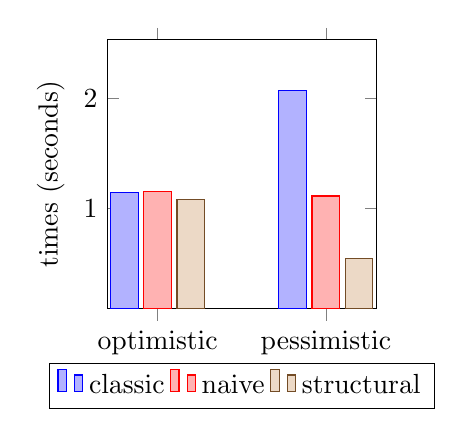
\begin{tikzpicture}
\begin{axis}[
    ybar,
    enlargelimits=0.3,
    width=5cm, height=5cm,
    legend style={at={(0.5,-0.2)},
      anchor=north,legend columns=-1},
    ylabel={times (seconds)},
    symbolic x coords={optimistic, pessimistic},
    xtick=data
    ]
\addplot coordinates {(optimistic,1.142) (pessimistic,2.073)};
\addplot coordinates {(optimistic,1.151) (pessimistic,1.110)};
\addplot coordinates {(optimistic,1.077) (pessimistic,0.542)};
\legend{classic,naive,structural}
\end{axis}
\end{tikzpicture}
  \caption{The results of revers$^o$ evaluation for a list with a length of 90}
  \label{fair:plot-reverso}
\end{figure}

\begin{figure}[h]
\centering
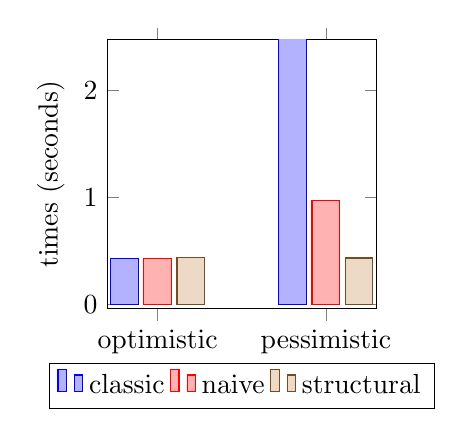
\begin{tikzpicture}
\begin{axis}[
    ybar, ymax = 2,
    enlargelimits=0.3,
    width=5cm, height=5cm,
    legend style={at={(0.5,-0.2)},
      anchor=north,legend columns=-1},
    ylabel={times (seconds)},
    symbolic x coords={optimistic, pessimistic},
    xtick=data
    ]
\addplot coordinates {(optimistic,0.430) (pessimistic,300)};
\addplot coordinates {(optimistic,0.428) (pessimistic,0.969)};
\addplot coordinates {(optimistic,0.433) (pessimistic,0.432)};
\legend{classic,naive,structural}
\end{axis}
\end{tikzpicture}
\caption{The results of sort$^o$ evaluation for a list with a length of 5}
\label{fair:plot-sorto}
\end{figure}

\begin{figure}[h]
\centering
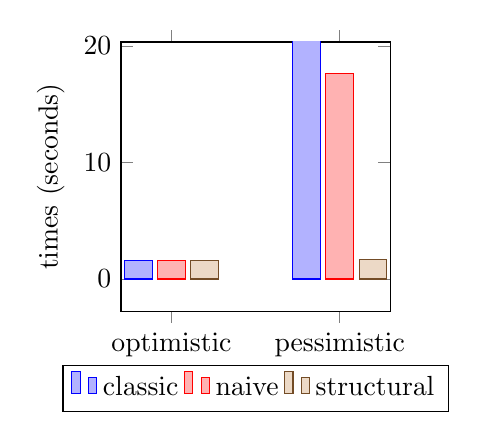
\begin{tikzpicture}
\begin{axis}[
    ybar, ymax = 16,
    enlargelimits=0.3,
    width=5cm, height=5cm,
    legend style={at={(0.5,-0.2)},
      anchor=north,legend columns=-1},
    ylabel={times (seconds)},
    symbolic x coords={optimistic, pessimistic},
    xtick=data
    ]
\addplot coordinates {(optimistic,1.574) (pessimistic,300)};
\addplot coordinates {(optimistic,1.579) (pessimistic,17.604)};
\addplot coordinates {(optimistic,1.585) (pessimistic,1.646)};
\legend{classic,naive,structural}
\end{axis}
\end{tikzpicture}
\caption{The results of ``The Tower of Hanoi'' solver}
\label{fail:plot-hanoi}
\end{figure}

\begin{figure}[h]
\centering
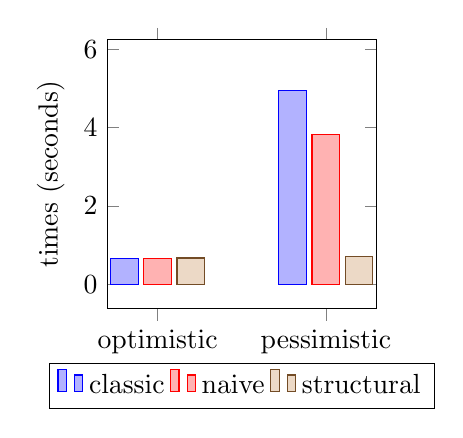
\begin{tikzpicture}
\begin{axis}[
    ybar,
    enlargelimits=0.3,
    width=5cm, height=5cm,
    legend style={at={(0.5,-0.2)},
      anchor=north,legend columns=-1},
    ylabel={times (seconds)},
    symbolic x coords={optimistic, pessimistic},
    xtick=data
    ]
\addplot coordinates {(optimistic,0.669) (pessimistic,4.956)};
\addplot coordinates {(optimistic,0.663) (pessimistic,3.820)};
\addplot coordinates {(optimistic,0.675) (pessimistic,0.712)};
\legend{classic,naive,structural}
\end{axis}
\end{tikzpicture}
\caption{The results of ``Bridge and torch problem'' solver}
\label{fair:plot-bridge}
\end{figure}

\begin{figure}[h]
  \small
  \centering
  \begin{tabular}{ c | c | c | c | c | c | c | c }
    \multirow{2}{*}{relation} & \multirow{2}{*}{size} & 
    \multicolumn{2}{c}{classic conjunction} &
    \multicolumn{2}{c}{naive fair conjunction} &
    \multicolumn{2}{c}{fair conjunction} \\
    \cline{3-8}
    & & optimistic & pessimistic & optimistic & pessimistic & optimistic & pessimistic  \\ 
    \hline
    \multirow{3}{*}{revers$^o$}
                 & 30   & 0.465 & 0.532 & 0.468 & 0.461  & 0.438 & 0.425 \\
                 & 60   & 0.579 & 0.828 & 0.577 & 0.658  & 0.545 & 0.450 \\
                 & 90   & 1.142 & 2.073 & 1.151 & 1.110  & 1.077 & 0.542 \\
    \hline
    \multirow{5}{*}{sort$^o$}
                 & 3    & 0.418 & 0.432 & 0.420 & 0.420  & 0.424 & 0.425 \\
                 & 4    & 0.424 & 3.924 & 0.424 & 0.455  & 0.429 & 0.429 \\
                 & 5    & 0.430 & >300  & 0.428 & 0.969  & 0.433 & 0.432 \\
                 & 6    & 0.434 & >300  & 0.430 & 11.577 & 0.434 & 0.437 \\
                 & 30   & 1.664 & >300  & 1.636 & >300   & 1.723 & 1.751 \\ 
    \hline
    hanoi$^o$    & -    & 1.574 & >300  & 1.579 & 17.604 & 1.585 & 1.646 \\
    \hline
    bridge$^o$   & -    & 0.669 & 4.956 & 0.663 & 3.820 & 0.675 & 0.712    

  \end{tabular}
  \caption{The results of an evaluation: running times of benchmarks in seconds}
  \label{fair:evaluation-table}
\end{figure}
\section{Conclusion}

% В данной работе мы предложили новый подход к исполнению реляционных программ со структурной рекурсией. Данный подход снижает влияние порядка конъюнктов на эффективность исполнения.
In this paper, we proposed a new approach to the execution of relational programs with structural recursion. This approach reduces the impact of conjunct order on performance.

% В дальнейшем мы планируем обобщить предложенный подход для большего класса программ. Также мы планируем формализовать наш подход в системе COQ и доказать, что сходимость вычисления не зависит от порядка конъюнктов.
In the future, we plan to generalize the proposed approach for a larger class of programs. We also plan to formalize our approach in the COQ~\cite{fair:Coq} system and prove that the convergence of the execution does not depend on the order of the conjuncts.

\bibliographystyle{ACM-Reference-Format}
\bibliography{fair-conj}


\end{document}
\endinput

